\section{Trải nghiệm người dùng}

\begin{figure}[H]
    \centering
    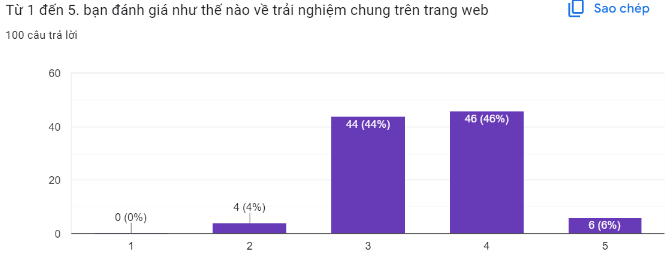
\includegraphics[width=0.8\linewidth]{images/survey1.png}
    \vspace{0.6cm}
    \caption{Khảo sát trải nghiệm chung về hệ thống}
\end{figure}

Từ hình 6.1 ta có, điểm trung bình khi hỏi về trải nghiệm chung của trang web rơi vào 3.54 trên tổng số 5 điểm. 3-4 điểm là mức điểm trung bình khác và vẫn có 4 nhận xét cho mức 2 điểm là tương đối tệ, cho thấy trang web cần cải thiện hơn, bổ sung tính năng về nhiều mặt để có thể hoàn thiện hơn nữa. Vì đây chỉ là demo cho thuật toán nên nhóm chưa đi vào khảo sát sâu hơn các phương diện khác đối với trải nghiệm người dùng. 

Về thuật toán giải quyết chính cho hệ hỗ trợ ra quyết định, như các phần trên nhóm đã trình bày thì nhóm sử dụng 2 thuật toán Weighted-sum và VIKOR. Tuy nhiên, Weighted-sum chỉ là thuật toán sơ cấp ban đầu được nhóm đề ra và khi khảo sát ban đầu không đem lại hiệu quả do đó nhóm quyết định chỉ thực hiện khảo sát trên VIKOR và đem lại một số điểm tích cực sau. 

Trong 3 gợi ý của hệ thống, số gợi ý mà các bạn sinh viên cảm thấy phù hợp hoặc chính xác chiếm tỉ lệ khoảng 69,33\%, đây cũng có thể xem như là độ chính xác của hệ thống gợi ý, ngoài ra các chỉ số khác như là \textbf{MSE} (Mean squared error) là 4,85, \textbf{MAE} (Mean absolute error) là 2,05, \textbf{RMSE} (Root mean squared error) là 2,202 và \textbf{MAPE} (Mean absolute percentage error) là 0.3 \cite{thu}. Với những chỉ số này thì kết quả của hệ thống vẫn được coi là chấp nhận được.
\begin{figure}[H]
    \centering
    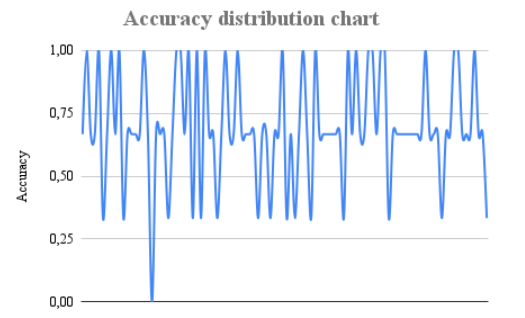
\includegraphics[width=0.6\linewidth]{images/accChart.png}
    % \vspace{0.6cm}
    % \caption{}
\end{figure}

Tuy vậy, khi khảo sát trên 100 sinh viên vẫn còn trường hợp sinh viên không thấy bất kì lựa chọn nào là phù hợp hơn nữa độ chính xác cũng phân bố không đều, do đó khảo sát này chỉ mang tính đại diện kết quả ban đầu.

Lấy kết quả gợi ý này so sánh với kết quả gợi ý của một số hệ thống lớn và hệ thống gợi ý trong các nghiên cứu liên quan, ta có được một kết quả so sánh tạm thời như sau đây.
\begin{figure}[H]
    \centering
    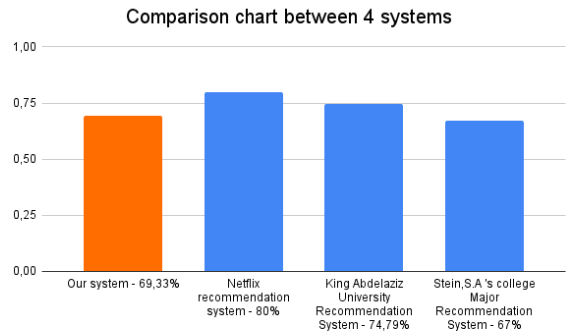
\includegraphics[width=0.6\linewidth]{comparisonChart.png}
    % \vspace{0.6cm}
    % \caption{}
\end{figure}

Nhìn chung đây là một kết quả có thể tạm chấp nhận được, khi so sánh với hệ thống gợi ý của Netflix hay so với một số hệ thống gợi ý được đưa ra ở \hyperref[2.2]{phần 2.2}, tuy vậy nếu so sánh thì ta có thể thấy rằng vẫn cần phải làm rất nhiều thứ phải làm để cải thiện hơn nữa độ chính xác của hệ thống, cũng như điều chỉnh để phù hợp hơn với tình hình kinh tế, xã hội ở Việt Nam.